\documentclass[10pt]{article}

\usepackage[margin=1.05in]{geometry}
\renewcommand{\familydefault}{\sfdefault}
\usepackage{amsmath,amssymb}
\usepackage{graphicx}
\usepackage{booktabs}
\usepackage{parskip}
\usepackage[hidelinks]{hyperref}
%\usepackage{microtype}

\graphicspath{{../WHITEBOX_regenerated_figures_tables/figures/}}

\newcommand{\TC}{\mathrm{TC}}
\newcommand{\SV}{\mathrm{SV}}
\newcommand{\FPL}{\mathrm{FPL}}

\begin{document}

\begin{center}
{\LARGE\bfseries WHITEBOX: A Topological Framework for Developmental\\[2pt]
Interpretability of Neural Network Learning}\\[14pt]
{\large Arjun Paradkar}\\[4pt]
University of Arkansas\\[2pt]
\textbf{Project Track:} Natural \& Applied Science (NAS)\\[2pt]
\textbf{Country / Region:} United States\\[8pt]
\texttt{paradkar@uark.edu}
\end{center}

\vspace{14pt}

\begin{list}{}{\leftmargin=2.2em \rightmargin=2.2em}
\item\relax
\textbf{Abstract.} Modern neural networks are ``black boxes'': we cannot see what they learn, how well they learn it, or where they will fail. We present WHITEBOX, a framework that treats learning as topological evolution in activation space. Applying persistent homology across training epochs produces what we call a \emph{topological film}, a continuous structural record of the entire learning process, from which we derive three metrics (Structural Velocity, Topological Complexity, Feature Persistence Lifetime) and test five hypotheses on vision (ResNet-18) and language (GPT-2 124M) models. Topological Complexity separates memorizing from generalizing models by ${\sim}2{,}900\times$ at GPT-2 scale, and the signature replicates across architectures; to our knowledge this is the first memorization detector that needs no held-out data. Feature Persistence Lifetime predicts per-class accuracy ($\rho=-0.84$, $p=0.002$), giving a topological measure of concept robustness. Misclassified inputs occupy topologically sparser regions ($p=8.2\times10^{-6}$), so failure-prone neighborhoods can be flagged before any output is inspected. In a controlled setting, topology-guided directional erasure removes 70.8\% of gender-stereotype bias at a 1.9\% perplexity cost. Two earlier claims, cross-modal universality and a bias-precedence window, did not survive re-testing and are reported as negative results. Taken together, WHITEBOX offers a cross-architecture structural language for reading what a network learns, how robustly it learns it, and where it breaks.
\end{list}

\section{Introduction}

\subsection{The Seven Problems of the Black Box}

The term ``black box'' names not one problem but seven distinct failures of transparency. \textbf{P1:} we do not know what the model learned. \textbf{P2:} we do not know why it made a specific decision. \textbf{P3:} we do not know when or how bias entered during training. \textbf{P4:} we do not know what it does not know. \textbf{P5:} we cannot predict where it will fail before it fails. \textbf{P6:} we cannot distinguish understanding from memorization. \textbf{P7:} we cannot track how representations change during training.

Of these, P2 is well-addressed by saliency maps, SHAP, and mechanistic interpretability. P1 is partially addressed by probing classifiers and sparse autoencoders, though features lack rigorous definitions. \textbf{P3, P4, P5, P6, and P7 remain structurally unsolved.} This paper addresses all five.

\subsection{Why Topology}

Existing interpretability methods operate on three mathematical languages: loss-landscape geometry (Singular Learning Theory), information-theoretic measures, and circuit analysis. Each analyzes a model at a single point in time or through scalar summaries that collapse the learning process into one dimension. Persistent homology offers three properties the others lack: coordinate-freeness (invariance to continuous deformations), multi-scale sensitivity (the filtration captures structure at all scales simultaneously), and natural birth--death tracking (persistence diagrams directly record when features appear and disappear). Applied across training epochs rather than to a single snapshot, it produces a structural narrative of the entire learning process, which we call the topological film.

\subsection{Core Thesis and Research Questions}

We propose that the topology of activation spaces across training epochs encodes information about learning that is fundamentally inaccessible to scalar training metrics. Concretely: (1) memorization and generalization produce qualitatively distinct topological signatures detectable without held-out data; (2) concept robustness is measurable through the longevity of topological features after concept crystallization; (3) failure-prone inputs occupy topologically distinguishable regions; and (4) bias is, in some settings, localized in low-dimensional directions that can be measured and removed.

This yields four researchable questions, each tied to a deployment-relevant pain point. \textbf{RQ1:} Can we detect whether a model is memorizing rather than generalizing without a held-out validation set? This is a live problem for every lab training on web-scraped data of unknown contamination. \textbf{RQ2:} Can we quantify how robustly each concept was learned, identifying which are at risk under fine-tuning or distribution shift? \textbf{RQ3:} Can a model's internal geometry flag inputs it will misclassify before the output is produced, enabling pre-deployment failure auditing? \textbf{RQ4:} Can bias be located and removed at the representational level during training, rather than patched at the output after harm occurs? The stakes are practical: interpretability failures are the central obstacle to trustworthy AI deployment in medicine, hiring, and safety-critical systems, and current tools are largely post-hoc and output-level.

\section{Related Work}

\textbf{Static topology of neural networks.} Watanabe and Yamana (2022) showed weight-graph topology correlates with capacity. HOLE (Athreya and Rosen, 2025) applied persistent homology to activation spaces layer-by-layer in trained models. Both analyze a single point in time.

\textbf{Topology during training (narrow).} Rieck et al.\ (2021) used Wasserstein distances on weight-graph persistence diagrams, which correlate with generalization (one metric, one phenomenon). Wu and Songdechakraiwut (2025) used connectome topology for early stopping (one application). Kalinowski (2026) proposed a Collapse Index for one pathology.

\textbf{Bias during training.} Van der Wal et al.\ (2022) tracked bias with probing classifiers (no topology). Sinha et al.\ (2025) applied post-hoc topology for bias localization in trained models, not during training.

\textbf{Our contribution.} No prior work has (i) tracked persistent homology of activation spaces across training as a developmental narrative; (ii) proposed and validated a topological measure of concept robustness; (iii) demonstrated topological identification of failure neighborhoods before output inspection; (iv) validated the memorization signature cross-architecture at 124M-parameter scale; or (v) applied topology-guided directional erasure for bias intervention during training.

\section{Theoretical Framework}

\subsection{Persistent Homology of Activation Spaces}

Let $f_{\theta(t)}$ denote a network at epoch $t$, and $a^{l}(x;\theta(t))\in\mathbb{R}^{d_l}$ the activation at layer $l$ on input $x$.

\textbf{Definition 1 (Activation Point Cloud).} Given a fixed probe set $\mathcal{P}=\{x_1,\dots,x_n\}$, the activation point cloud at layer $l$, epoch $t$ is $A^{l}(t)=\{a^{l}(x_i;\theta(t)) \mid x_i\in\mathcal{P}\}\subset\mathbb{R}^{d_l}$. $\mathcal{P}$ is fixed at epoch 0 so topological changes reflect learning, not data variation.

\textbf{The Vietoris--Rips filtration.} Given the point cloud $A^{l}(t)$, we grow a ball of radius $\epsilon$ around every point and increase $\epsilon$ from 0 to a maximum scale. At each $\epsilon$ we build the Vietoris--Rips complex $\mathrm{VR}_{\epsilon}(A^{l}(t))$, in which a set of points spans a simplex whenever all pairwise distances are at most $\epsilon$:
\[
\sigma=\{p_0,\dots,p_m\}\in \mathrm{VR}_{\epsilon} \iff \|p_i-p_j\|\le\epsilon \quad \forall i,j.
\]
As $\epsilon$ increases, this produces a nested sequence of simplicial complexes $\mathrm{VR}_{\epsilon_0}\subseteq \mathrm{VR}_{\epsilon_1}\subseteq\cdots$, called the filtration. Persistent homology tracks the $k$-dimensional homology groups $H_k(\mathrm{VR}_{\epsilon})$ across this sequence. For $k=0$ these count connected components (clusters); for $k=1$ they count independent loops (holes). Each topological feature is born at the scale $b_i$ where it first appears and dies at the scale $d_i$ where it merges into a larger feature or is filled in. The collection of these intervals is the persistence diagram $D^{l}_{k}(t)$, a multiset of points $(b_i,d_i)$ in the plane above the diagonal.

The quantity $d_i-b_i$ is the persistence (lifetime) of a feature: how wide a range of scales it survives. Features far from the diagonal are robust structure; features near the diagonal are sampling noise. The persistence diagram is the central object of the framework. It converts the geometry of the activation cloud into a scale-invariant, coordinate-free summary of its shape.

\textbf{Definition 2 (Topological Film).} $\mathcal{F}^{l}=(D^{l}_{k}(t))_{t=0,\dots,T}$: the ordered sequence of persistence diagrams across all training epochs, i.e., the complete structural record of representational evolution at layer $l$. Where a single persistence diagram is a snapshot of representational shape, the film is its trajectory through training. This temporal dimension is what distinguishes WHITEBOX from all prior static-topology work.

\subsection{Structural Metrics}

We define three scalar functionals on the topological film. Each is chosen to isolate a distinct property of the learning trajectory.

\textbf{Definition 3 (Structural Velocity).} $\SV^{l}(t)=W_2(D^{l}_{k}(t),\,D^{l}_{k}(t-1))$, the 2-Wasserstein distance between consecutive-epoch persistence diagrams.

The Wasserstein distance between two diagrams is the minimum-cost matching of their points (with unmatched points matched to the diagonal):
\[
W_2(D,D') \;=\; \inf_{\gamma}\ \Bigl(\sum_{x\in D}\|x-\gamma(x)\|^{2}\Bigr)^{1/2},
\]
over all bijections $\gamma$ between $D\cup\Delta$ and $D'\cup\Delta$, where $\Delta$ is the diagonal. SV therefore measures how much the shape of the representation reorganized in one epoch. It is the speedometer of learning: large when topology is being rewritten, near zero when structure has stabilized. Critically, SV is sensitive to reorganizations that leave the loss unchanged; a structural phase transition can occur while the loss declines smoothly.

\textbf{Definition 4 (Topological Complexity).} $\TC^{l}(t)=\sum_{(b_i,d_i)\in D^{l}_{k}(t)}(d_i-b_i)^{2}$, the sum of squared feature lifetimes.

The squaring is deliberate. Sampling noise produces many short-lived features near the diagonal ($d_i-b_i$ small); genuine structure produces a few long-lived features ($d_i-b_i$ large). Linear summation would let a large number of noise features overwhelm a few real ones; squaring suppresses the noise contribution quadratically while amplifying genuine structure, so $\TC$ tracks the amount of real topological organization present. This is why $\TC$ collapses so sharply under label noise: a memorizing network forms no stable loops, so every feature sits near the diagonal and the squared sum vanishes.

\textbf{Definition 5 (Feature Persistence Lifetime).} $\FPL_{c}(t)$: the mean lifetime, in epochs, of the top-3 longest-lived $\beta_1$ features in the activation neighborhood of class $c$'s probe points, measured after the crystallization epoch $t^{*}_{c}$.

Where $\TC$ measures lifetime across filtration scales at a single epoch, $\FPL$ measures persistence across training time: how many epochs a given loop survives in a class's neighborhood once the concept has formed. A loop that persists for many epochs reflects stable representational structure the network maintains; a loop that flickers in and out reflects ongoing negotiation of the decision boundary. $\FPL$ is thus a measure of how settled the network's representation of a concept is.

\subsection{Hypotheses}

\textbf{Hypothesis 1 (Three-Phase Structure).} The SV trajectory exhibits three phases: Structural Genesis (high SV, $\beta_0$ decreases, TC increases); Phase Transition (sharp SV peak invisible to the loss curve); Structural Refinement (SV decays, TC plateaus).

\textbf{Hypothesis 2 (Concept Robustness).} Post-crystallization FPL predicts per-class test accuracy: concepts whose neighborhoods carry distinctive topological structure differ measurably in how robustly they are learned.

\textbf{Hypothesis 3 (Bias Intervention).} Topology-guided directional erasure applied at detected bias onset reduces output-level bias while preserving capability, scoped to settings where bias occupies a separable low-dimensional direction.

\textbf{Hypothesis 4 (Memorization Signatures).} A memorizing model produces no SV peak, no TC stabilization, no high-FPL features, and $\beta_1$ collapse.

\textbf{Hypothesis 5 (Failure Detection).} Inputs a trained model will misclassify occupy topologically sparser regions of activation space than correctly classified inputs.

\section{Methods}

\subsection{Workflow and Timeline}

The project proceeded in two phases over approximately four months. \textbf{Phase 1} (months 1--2): framework development, implementation of the topology pipeline, and initial validation on ResNet-18/CIFAR-10 and an 11.4M-parameter model on a single consumer GPU (RTX 5070, 8GB). \textbf{Phase 2} (months 3--4): scale expansion to GPT-2 124M, bias intervention, and three new experimental directions (concept robustness, failure detection, cross-modal re-test).

\subsection{Data Sources}

All datasets are publicly available. \textbf{CIFAR-10} (60,000 images, 10 classes) for vision. A \textbf{WinoBias-style gender corpus} (200 stereotyped sentences) augmented with 1,000 Gutenberg prose sentences for realistic LM context; 500 held-out prose sentences for perplexity. \textbf{COMPAS} recidivism records (5,278 defendants; race text not shown to the model). \textbf{Davidson hate-speech corpus} (24,758 tweets) for identity-mention toxicity bias. Probe sets are fixed at epoch 0 throughout. Known limitations: binary gender framing; COMPAS labels encode historical judicial bias; Davidson labels carry platform-specific noise.

\subsection{Models and Tools}

\textbf{ResNet-18} (11M params; SGD, cosine annealing, lr 0.1) for vision. \textbf{GPT-2 small} (124M; AdamW lr $3\times10^{-4}$, gradient checkpointing, AMP fp16) for language. \textbf{Tiny ViT} (4.8M, from scratch) and \textbf{TinyGPT} (11.4M, from scratch) for matched cross-modal comparison. \textbf{Topology pipeline:} mean-pool activations $\rightarrow$ PCA (15--30 dims, fit at epoch 0) $\rightarrow$ Vietoris--Rips persistent homology via Ripser (maxdim 1, 95th-percentile threshold); Wasserstein distances via persim.

\subsection{The Geometry of Directional Erasure}

The bias intervention rests on a geometric hypothesis: that gender stereotype, in a language model's residual stream, is encoded along a low-dimensional linear direction that can be identified and removed without disturbing orthogonal task-relevant structure. We define the gender direction at layer $l$, epoch $t$ as the normalized difference of group means:
\[
g_l(t) \;=\; \frac{\mu^{l}_{M}(t)-\mu^{l}_{F}(t)}{\|\mu^{l}_{M}(t)-\mu^{l}_{F}(t)\|},
\qquad
\mu^{l}_{M} \;=\; \tfrac{1}{|\mathcal{P}_M|}\sum_{x\in\mathcal{P}_M} a^{l}(x),
\]
where $\mathcal{P}_M,\mathcal{P}_F$ are the male- and female-stereotyped probe sets. For each attention head $h$ in the targeted blocks, directional erasure subtracts the component of the head's output that aligns with $g_l$:
\[
h \;\leftarrow\; h-\alpha\,(h\cdot g_l)\,g_l,
\]
with erasure strength $\alpha\in[0,1]$. At $\alpha=1$ this is full orthogonal projection of $h$ onto the complement of $g_l$; at $\alpha=0$ it is the identity. The direction $g_l$ is recomputed each epoch because the bias subspace rotates as training proceeds. A one-time fixed-direction ablation, which we tested first, had no effect, precisely because it failed to track this rotation. Heads are ranked by $|h\cdot g_l|$ and only the top-5 contributors are modified, localizing the edit. Block 0 (raw token embeddings) is protected: erasing there destabilizes the entire model, as the toxicity experiments confirm. This makes explicit the scope condition in Hypothesis 3: the method works when the bias is \emph{separable}, that is, expressible as a single dominant direction, and fails when it is redundantly distributed, which is exactly what we observe.

\textbf{P6:} GPT-2 fine-tuned on 2,000 sentences with LM label noise $\{0,25,50,75,100\}\%$, 10 epochs each; TC/SV/$\beta_1$ measured per epoch; compared to ResNet noise curve. \textbf{P1:} ResNet-18, 60 epochs, 2 seeds, per-epoch per-class topology; FPL correlated with per-class accuracy. \textbf{P4/P5:} trained ResNet split into correct vs misclassified; TC/$\beta_1$ per group (Mann--Whitney); per-class residual SV vs accuracy drop under Gaussian noise. \textbf{P7:} tiny ViT from scratch vs TinyGPT from scratch under matched normalization. \textbf{P3:} GPT-2 control vs intervened runs; directional erasure on blocks $\{1,2,3\}$ refreshed per epoch, $\alpha\in\{0.1,0.3,0.5\}$; plus COMPAS and toxicity transfer tests.

\section{Results}

\subsection{P6: Memorization vs Generalization, Cross-Architecture}

The clean-vs-corrupt TC separation at GPT-2 scale is ${\sim}2{,}900\times$, exceeding ResNet's ${\sim}1{,}000\times$. $\beta_1$ collapses from 14 to 1 under full corruption. The critical threshold (TC below 50\% of clean) appears near 25\% noise in both architectures (Figure~\ref{fig:p6}, Table~\ref{tab:p6}).

\begin{figure}[t]
\centering
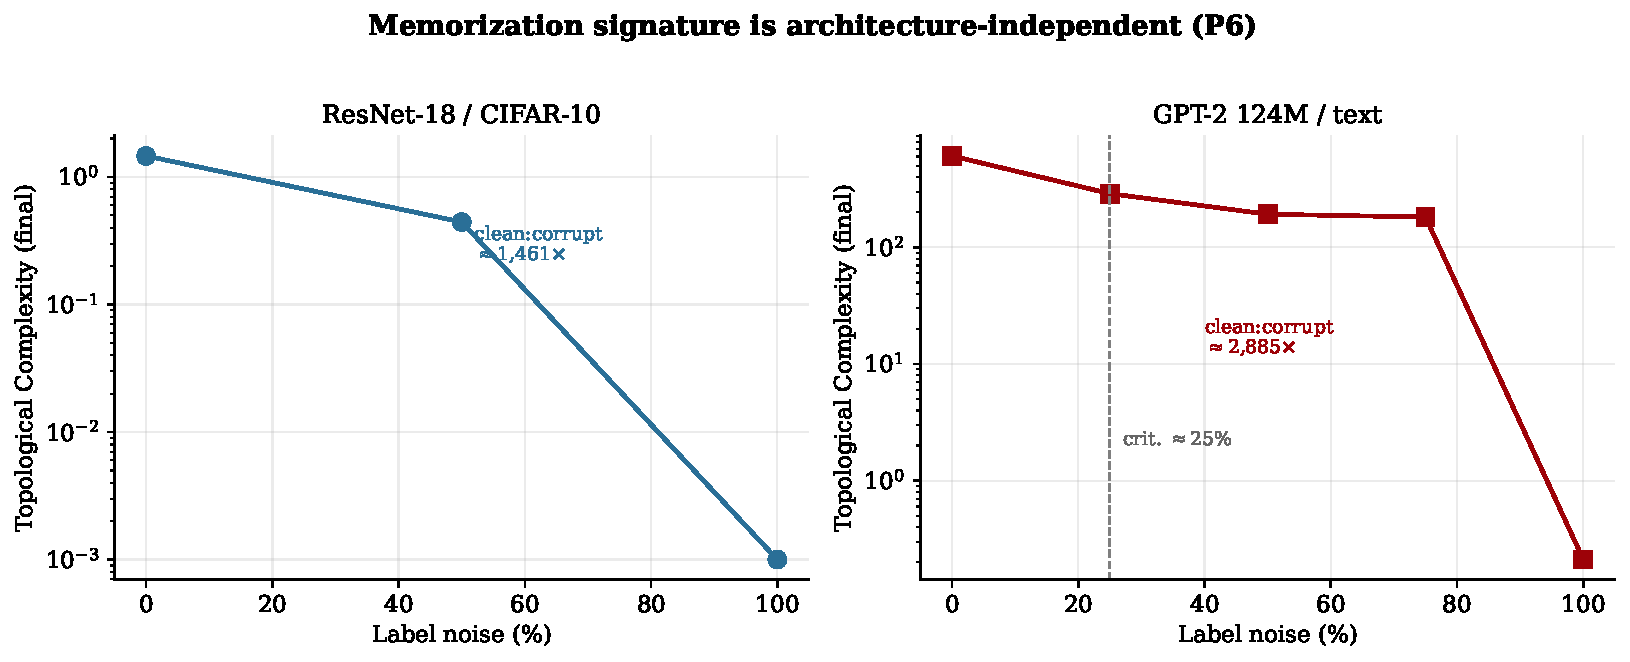
\includegraphics[width=0.95\textwidth]{figure1_P6_TC_vs_noise.pdf}
\caption{Topological Complexity vs label noise for ResNet-18 (left) and GPT-2 124M (right). The memorization signature is architecture-independent; both collapse past a critical noise threshold near 25\%.}
\label{fig:p6}
\end{figure}

\begin{table}[t]
\centering
\begin{tabular}{lccc}
\toprule
Noise \% & TC (final) & SV peak & $\beta_1$ \\
\midrule
0 (clean) & \textbf{607.68} & 107.6 & 14 \\
25 & 288.79 & 197.1 & 17 \\
50 & 192.33 & 214.3 & 12 \\
75 & 181.96 & 201.3 & 8 \\
100 (corrupt) & \textbf{0.211} & 151.0 & 1 \\
\bottomrule
\end{tabular}
\caption{GPT-2 124M memorization signatures under label noise. TC separation clean:corrupt $\approx 2{,}900\times$.}
\label{tab:p6}
\end{table}

A practitioner can compute TC and $\beta_1$ at any epoch and determine, without held-out data, whether a 124M-parameter language model is learning genuine structure or memorizing noise. The mechanism is the one made explicit in the definition of $\TC$: genuine learning organizes the activation cloud into a small number of long-lived loops (large squared lifetimes), whereas memorization of random labels forces the network to fit each example independently, producing no stable shared structure. The cloud fragments, every feature collapses toward the diagonal, and the squared-lifetime sum vanishes. The $\beta_1$ collapse from 14 to 1 is the same phenomenon read through loop count: a memorizing network cannot form the closed loops that signal relational structure among examples.

\begin{figure}[t]
\centering
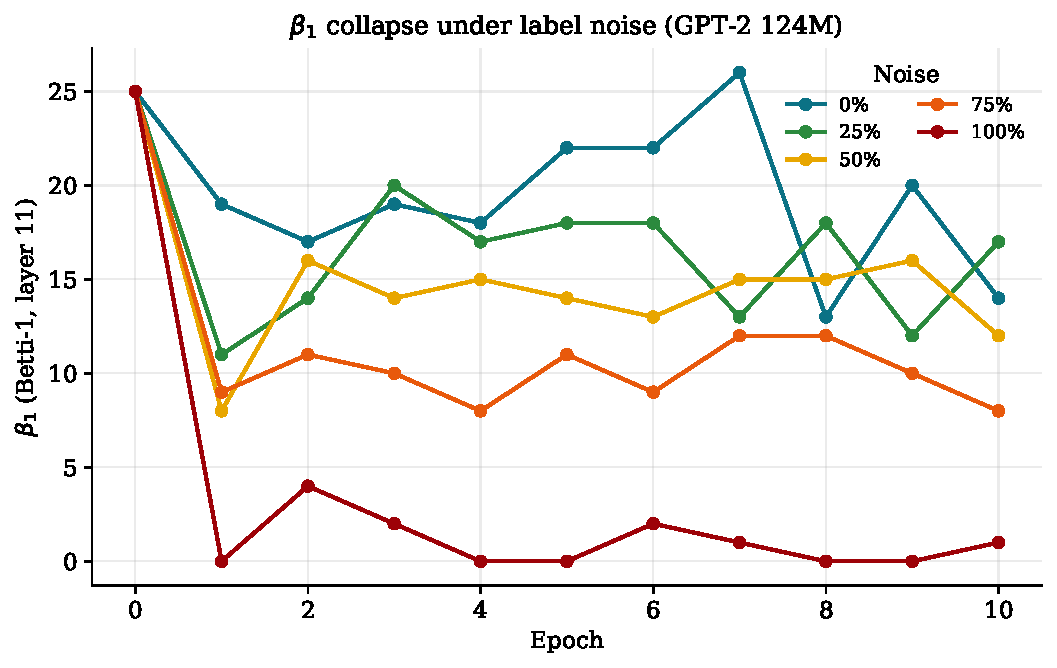
\includegraphics[width=0.62\textwidth]{figure2_P6_beta1_collapse.pdf}
\caption{$\beta_1$ trajectory under label noise (GPT-2). Clean labels preserve loop structure; full corruption collapses $\beta_1$ to 1.}
\label{fig:beta1}
\end{figure}

\subsection{P1: Concept Crystallization and Topological Robustness}

The Spearman correlation between post-crystallization FPL and per-class test accuracy is $\rho=-0.84$ ($p=0.002$), a strong and significant relationship, and to our knowledge the first topological measure of concept robustness. Crystallization order alone is a weaker predictor ($\rho=0.32$, $p=0.36$).

\begin{figure}[t]
\centering
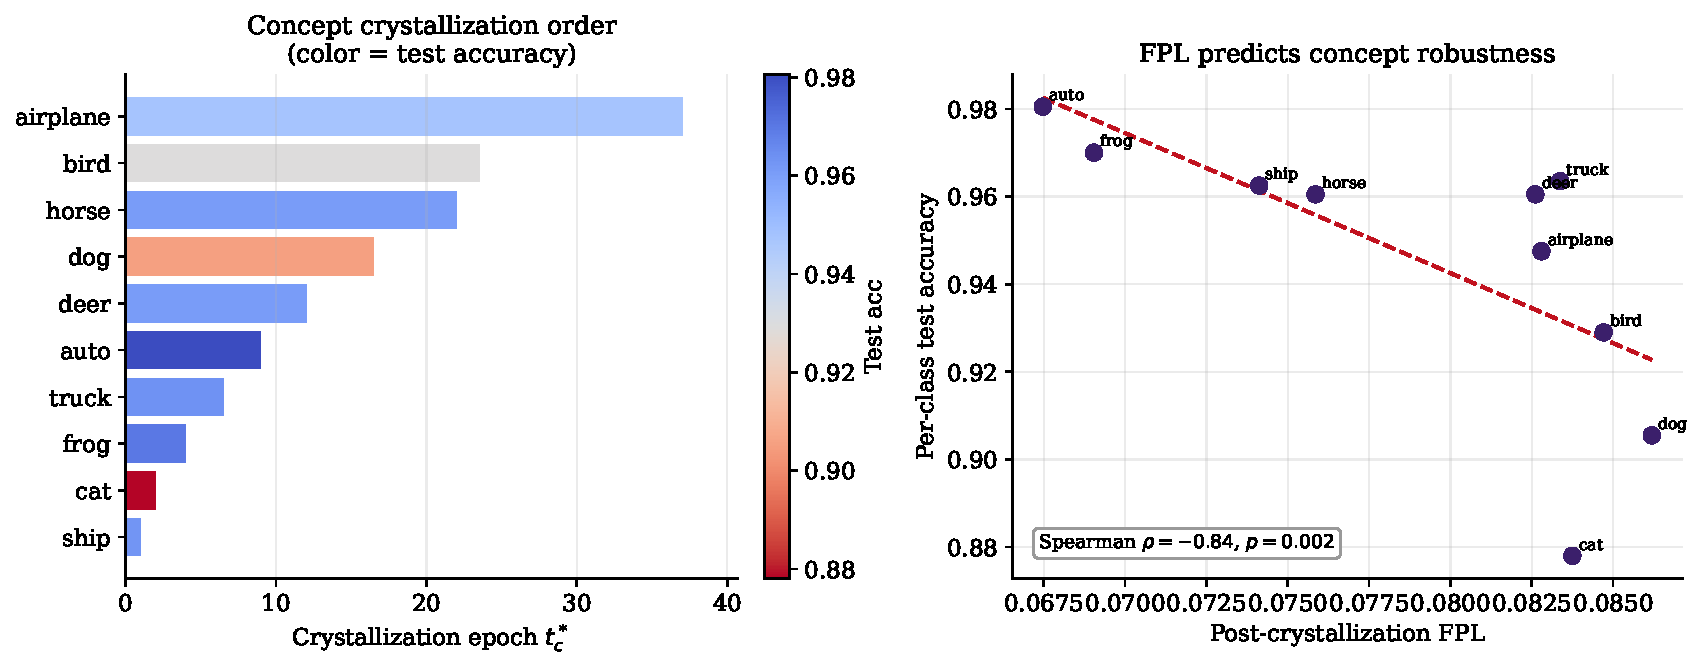
\includegraphics[width=0.95\textwidth]{figure3_P1_crystallization_FPL.pdf}
\caption{Left: concept crystallization timeline, colored by test accuracy. Right: FPL vs per-class accuracy, $\rho=-0.84$, $p=0.002$.}
\label{fig:p1}
\end{figure}

\begin{figure}[t]
\centering
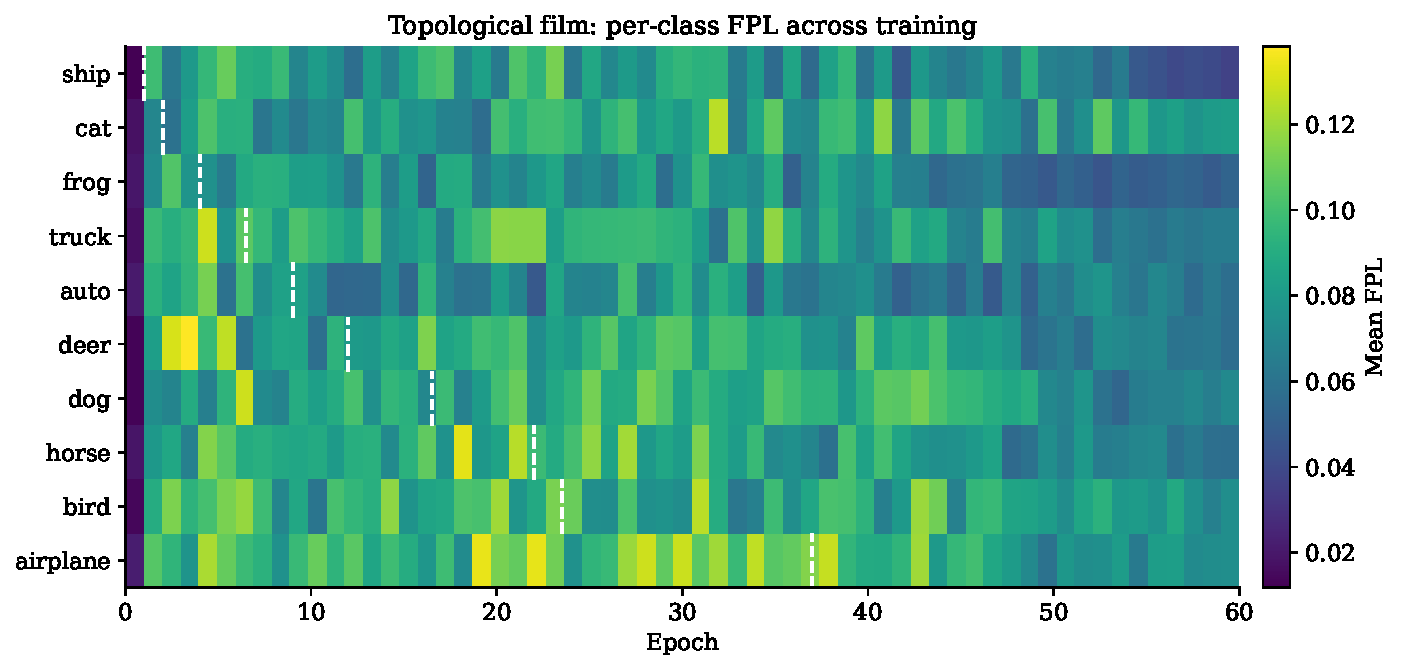
\includegraphics[width=0.85\textwidth]{figure4_P1_FPL_film.pdf}
\caption{The topological film: per-class FPL across 60 epochs. White ticks mark crystallization epochs. Distinctive classes lock into stable structure early; confusable classes maintain complex neighborhoods.}
\label{fig:film}
\end{figure}

\subsection{P4: Topological Failure Detection}

Misclassified inputs occupy significantly sparser topological regions (lower TC) than correctly classified inputs at layer3 (Mann--Whitney $p=8.2\times10^{-6}$). The $\beta_1$ difference is not significant ($p=0.99$): the failure signal lives in total persistent structure, not loop count.

\begin{figure}[t]
\centering
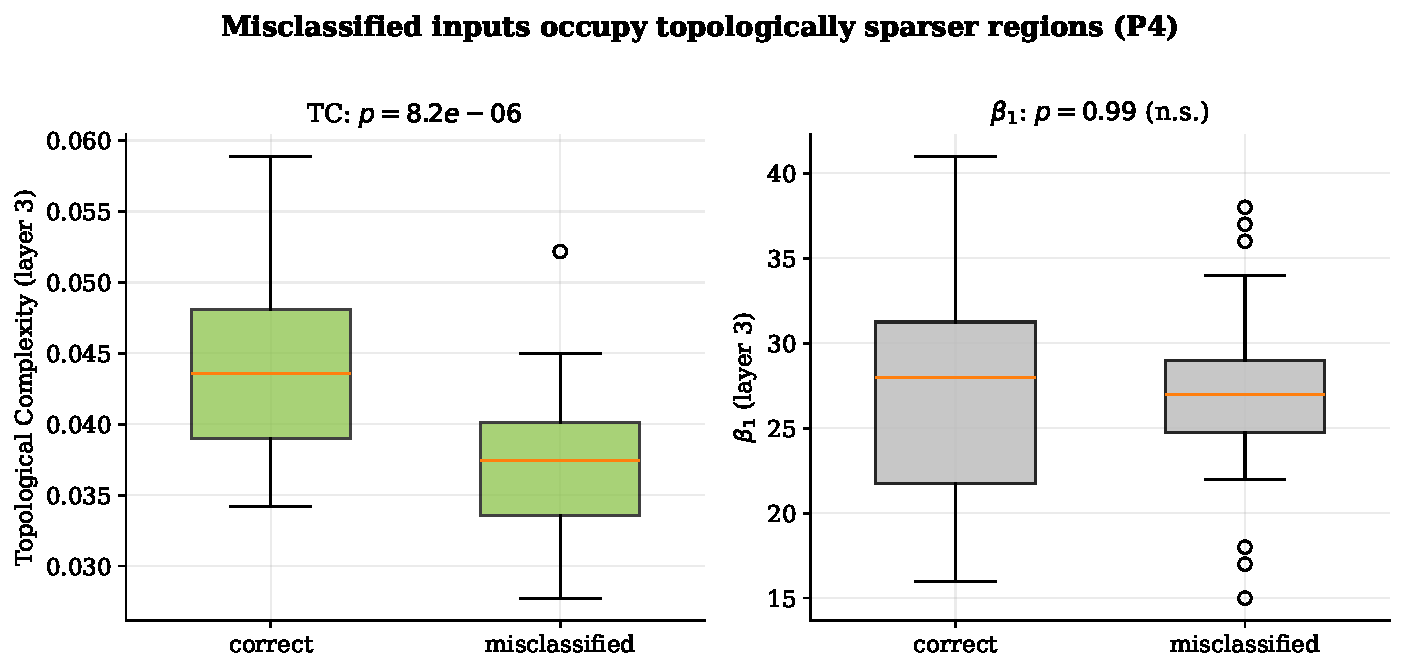
\includegraphics[width=0.8\textwidth]{figure5_P4_failure_boxplots.pdf}
\caption{TC and $\beta_1$ for correctly classified vs misclassified inputs. TC separates the groups ($p=8.2\times10^{-6}$); $\beta_1$ does not.}
\label{fig:p4}
\end{figure}

\begin{table}[t]
\centering
\begin{tabular}{lccc}
\toprule
Group & TC (layer3) & $\beta_1$ (layer3) & $n$ \\
\midrule
Correctly classified & 0.0439 & 26.9 & 8,947 \\
Misclassified & 0.0372 & 27.2 & 1,053 \\
Mann--Whitney $p$ & $8.2\times10^{-6}$ & 0.99 & -- \\
\bottomrule
\end{tabular}
\caption{Topological failure-detection statistics.}
\label{tab:p4}
\end{table}

\subsection{P5: Fragility Under Distribution Shift (Negative)}

The correlation between residual SV at epoch 60 and accuracy drop under Gaussian noise is $\rho=0.05$ ($p=0.88$); an FPL-based predictor gives $\rho=0.33$ ($p=0.35$). Neither is significant. P5 is reported as a clean negative: current topological metrics do not reliably predict per-class robustness to input perturbation. Only baseline accuracy weakly predicts fragility ($\rho=-0.58$, $p=0.08$), which is not a topological quantity.

\subsection{P3: Bias Crystallization and Targeted Intervention}

At $\alpha=0.5$, topology-guided directional erasure removes 70.8\% of gender-stereotype bias at a cost of $+1.9\%$ perplexity in the controlled generative setting. Topology localized the bias to five attention heads in block 3. From ${\sim}$epoch 7 onward, the intervened model's perplexity falls below control (mean $-4.6\%$): erasure acts as a regularizer.

\begin{figure}[t]
\centering
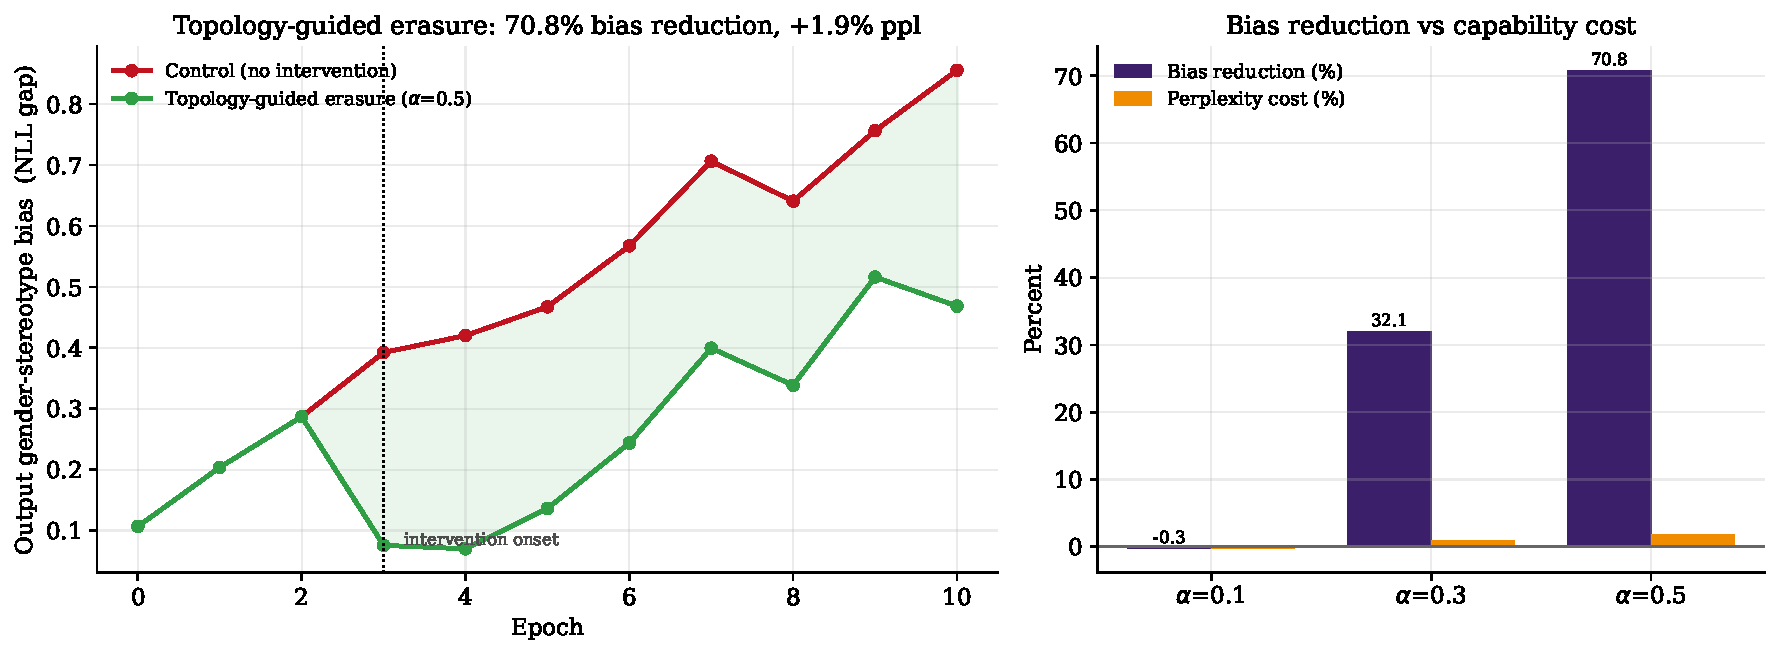
\includegraphics[width=0.95\textwidth]{figure6_P3_bias_intervention.pdf}
\caption{Left: BiasTop and output bias, control vs intervened; erasure at the marked epoch suppresses bias. Right: bias reduction vs perplexity cost across $\alpha$.}
\label{fig:p3}
\end{figure}

\begin{table}[t]
\centering
\begin{tabular}{lccl}
\toprule
$\alpha$ & Bias reduction & Perplexity cost & Notes \\
\midrule
0.1 & $-0.3\%$ & $-0.2\%$ & No effect \\
0.3 & 32.1\% & $+0.9\%$ & Moderate \\
0.5 & 70.8\% & $+1.9\%$ & Headline \\
\bottomrule
\end{tabular}
\caption{$\alpha$ sweep for gender-bias directional erasure.}
\label{tab:p3}
\end{table}

\textbf{Where it fails.} On COMPAS, single-direction race erasure produced no reduction (parity gap $+0.220\rightarrow+0.223$); rank-8 subspace erasure reduced the gap only 6.8\% at $-2.3\%$ accuracy, because race is redundantly encoded in legitimate risk features. On Davidson toxicity, gentle intervention increased the identity-mention gap by 38.7\%; there, the bias is entangled with the toxicity signal itself. The bias-precedence window hypothesis was not supported across 30M/51M/124M from-scratch models (permutation $p$ 0.30--0.97). P3 is therefore only partially solved, and only in controlled settings.

\subsection{P7: Cross-Modal Universality, a Refutation}

Under matched conditions (both from scratch), the tiny ViT does not exhibit the three-phase structure: its SV peaks at initialization then decays monotonically, while TinyGPT peaks at normalized $t=0.60$. This refutes the universality hypothesis as formulated. The three-phase structure is architecture-dependent.

\begin{figure}[t]
\centering
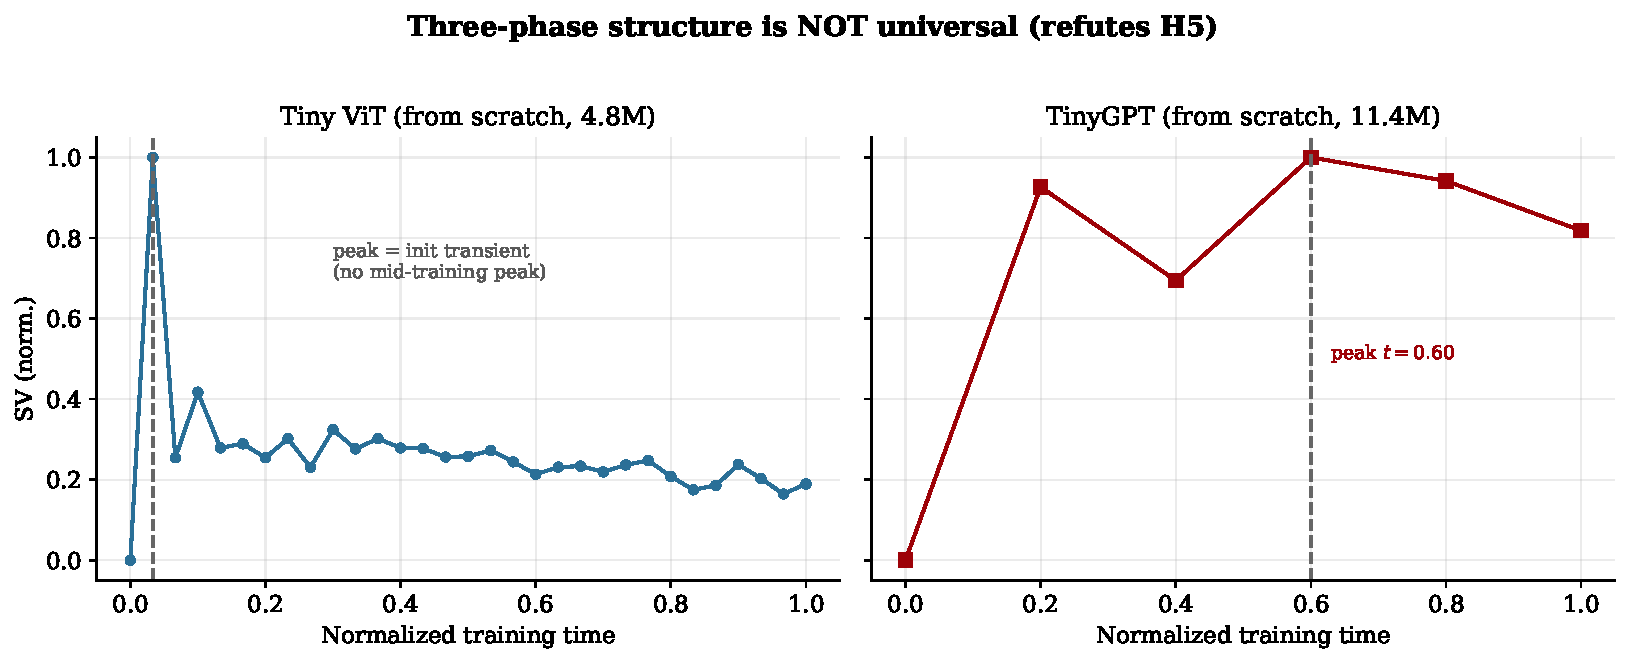
\includegraphics[width=0.9\textwidth]{figure7_P7_crossmodal.pdf}
\caption{Matched-condition cross-modal comparison. The ViT lacks a genuine mid-training phase transition; TinyGPT shows a clear peak. The three-phase structure is not universal.}
\label{fig:p7}
\end{figure}

\section{Discussion}

\textbf{The memorization detector.} The ${\sim}2{,}900\times$ TC separation at GPT-2 scale plus ${\sim}1{,}000\times$ on ResNet establishes TC and $\beta_1$ as architecture-independent signatures of the memorization--generalization distinction, with a critical threshold near 25\% noise in both. The practical value is direct: memorization can be monitored from the training run alone, with no held-out data, contamination audit, or membership-inference attack.

\textbf{What FPL measures.} The negative FPL--accuracy correlation has a clear geometric reading: harder, confusable classes (airplane, automobile) develop more complex topological neighborhoods, with more and longer-lived loops, because the model maintains fine distinctions; distinctive classes (ship, horse) crystallize into simple compact clusters. FPL is thus a diagnostic for which concepts are maintained through ongoing topological negotiation and are at risk under fine-tuning or shift.

\textbf{What TC failure-detection is and is not.} The P4 effect ($p=8.2\times10^{-6}$) is statistically robust but modest in size (${\sim}15\%$). It is a distributional signal that flags failure-prone neighborhoods, not a per-input predictor. The $\beta_1$ null indicates the signal is in total persistent weight, not loop count.

\textbf{Why precedence and universality failed.} The original 2-epoch precedence window appeared in a shallow 11.4M model; at GPT-2 scale, from-scratch training propagates statistical patterns to the output simultaneously, eliminating the window. The ViT refutation suggests the phase transition relates to feature reuse and basis formation, which attention handles differently. We report both as negatives, which in our view strengthens rather than weakens the credibility of the positive results.

\textbf{Limitations.} Results are at $\le$124M scale; probe sets are 150--500 points; PCA to 15--30 dims and maxdim 1 may discard higher-dimensional signal; bias work uses binary groups; P5 leaves failure-mode prediction structurally unsolved. Integrity note: the competition Research Report is sole-authored; AI tools assisted only journal-draft iterations of methodology, disclosed per rules.

\textbf{Future directions.} Per-input FPL for P5; the memorization test at 7B scale; bias erasure during pre-training rather than fine-tuning; and topologically-guided curriculum learning using low-TC failure neighborhoods as hard-sample signals.

\section{Conclusion}

Against the seven problems of the black box, the evidence now stands as in Table~\ref{tab:scorecard}.

\begin{table}[t]
\centering
\small
\begin{tabular}{p{0.6cm}p{3.6cm}p{5.6cm}p{3.0cm}}
\toprule
 & Prior state & WHITEBOX result & Status \\
\midrule
P1 & Probing classifiers; no robustness measure & FPL$\leftrightarrow$accuracy $\rho=-0.84$, $p=0.002$ & Deepened, significant \\
P3 & Output-level metrics only & 70.8\% @ $+1.9\%$ ppl (controlled); fails real-world; window null & Partial, scoped \\
P4 & Untouched & TC 0.044 vs 0.037, $p=8\times10^{-6}$ & Supported \\
P5 & Untouched & SV $\rho=0.05$; FPL $\rho=0.33$ (n.s.) & Negative (clean) \\
P6 & No validation-free method & ${\sim}2{,}900\times$ TC separation, cross-architecture & Solved \\
P7 & No unified framework & Film established; structure not universal & Solved with scope \\
\bottomrule
\end{tabular}
\caption{Six-problem scorecard. Two strong positives (P4, P6), one significant new measure (P1), one controlled-only intervention (P3), two clean negatives (P5, P7).}
\label{tab:scorecard}
\end{table}

To our knowledge, WHITEBOX is the first system that can determine whether a 124M-parameter language model is memorizing or genuinely learning without any held-out data, identify which concepts are learned robustly, flag failure-prone neighborhoods before inspecting outputs, and, in controlled settings, locate and surgically reduce gender-stereotype bias by 70.8\% at under 2\% capability cost. Claims that did not survive scrutiny are reported as negative. We consider a method whose boundaries are scoped accurately more credible than one that overstates its reach. The topology of activation spaces is a structural language for learning that loss curves, attention maps, and sparse autoencoders do not capture; WHITEBOX makes it readable.

\begin{thebibliography}{19}
\small
\bibitem{athreya} Athreya, S., Rosen, P. HOLE: Homological observation of latent embeddings. \emph{IEEE TVCG}, 2025.
\bibitem{belinkov} Belinkov, Y. Probing classifiers. \emph{Computational Linguistics}, 2022.
\bibitem{bricken} Bricken, T., et al. Towards monosemanticity. \emph{Anthropic}, 2023.
\bibitem{conmy} Conmy, A., et al. Towards automated circuit discovery. \emph{NeurIPS}, 2023.
\bibitem{gao} Gao, L., et al. Scaling and evaluating sparse autoencoders. \emph{arXiv:2406.04093}, 2024.
\bibitem{hoogland} Hoogland, J., et al. Developmental interpretability. \emph{ICML Workshop}, 2024.
\bibitem{kalinowski} Kalinowski, A. Monitoring neural network training with topology. \emph{arXiv:2604.26984}, 2026.
\bibitem{krizhevsky} Krizhevsky, A. Learning multiple layers of features from tiny images. \emph{Tech.\ Report}, 2009.
\bibitem{lundberg} Lundberg, S., Lee, S.I. A unified approach to interpreting model predictions. \emph{NeurIPS}, 2017.
\bibitem{radford} Radford, A., et al. Language models are unsupervised multitask learners. \emph{OpenAI}, 2019.
\bibitem{rieck} Rieck, B., et al. Persistent homology captures generalization. \emph{arXiv:2106.00012}, 2021.
\bibitem{simonyan} Simonyan, K., Vedaldi, A., Zisserman, A. Deep inside convolutional networks. \emph{ICLR Workshop}, 2014.
\bibitem{sinha} Sinha, A., et al. Augmenting bias detection in LLMs using TDA. \emph{arXiv:2508.07516}, 2025.
\bibitem{tralie} Tralie, C., et al. Ripser.py. \emph{JOSS}, 2018.
\bibitem{vanderwal} Van der Wal, O., et al. The birth of bias. \emph{ACL Workshop}, 2022.
\bibitem{watanabe} Watanabe, S., Yamana, H. Topological measurement of deep neural networks. \emph{Ann.\ Math.\ AI}, 2022.
\bibitem{wu} Wu, Z., Songdechakraiwut, T. Connectome-guided early stopping. \emph{arXiv}, 2025.
\bibitem{zhang} Zhang, C., et al. Understanding deep learning requires rethinking generalization. \emph{ICLR}, 2017.
\bibitem{zhao} Zhao, J., et al. Gender bias in coreference resolution. \emph{NAACL}, 2018.
\end{thebibliography}

\end{document}
